% !TEX root = ../pdf/stat205.tex
% [There are multiple stat205.tex files, but the one in ../pdf is the usual one]



%%%%%%%%%%%%%%%%%%%%%%%%%%%%%%%%%%%%%%%%%%%%%%%
\chapter{Probability and Risk~\label{ch:probandacc}}


\begin{verse}{\it
``When there are but two players, your theory which proceeds by combinations is very just. \\
But when there are three, I believe I have a proof that it is unjust that you should proceed in any other manner than the one I have.''\vspace*{6pt}} \\
\hspace*{2cm} -- Pascal's letter to Fermat\FOOTNOTE{from \url{https://www.york.ac.uk/depts/maths/histstat/pascal.pdf}}
\end{verse}
\vspace*{12pt}


\section{Indtroduction~\label{sec:intro}}

While scientists have always tried to understand the universe with technology and explain it with complete certainty, this is not always possible.
In other words, there is no other way but to accept chance as part of our lives.

The concept of chance has been extensively explored across elementary, professional, and philosophical literature, serving as a key motivation for our study.
While chance often appears unpredictable and devoid of structure, mathematicians have long sought to define it through rules and systematic frameworks.
Not surprisingly, gamblers were among the first to seek systematic frameworks for understanding their games - probing the mechanics of luck, wins and losses.
In 1654, a Parisian gambler named Antoine Gombaud (alias Chevalier de Méré), posed critical questions about winning probabilities to two of the era’s greatest mathematicians: Blaise Pascal and Pierre de Fermat.
Through their correspondence, the two mathematicians initiated the development of modern probability theory.
However, Gerolamo Cardano and Galileo Galilei, two Italian scholars, had also made significant contributions that captured the interest of Italian gamblers.

After years of development, the Russian mathematician Andrey Kolmogorov introduced the standard probability axioms in 1933, establishing the rigorous foundations of modern probability theory.
Today, probability theory serves as a fundamental tool across diverse fields including social sciences, medicine, biology, machine learning, physics, and countless other applications.
The following sections provide rigorous definitions of key concepts needed to establish a precise theoretical foundation.

\section{Random Experiment and Sample Space}

Suppose we want to conduct an experiment for which we know all possible outcomes.
Assuming the experimental conditions remain constant each time, if each realization of this experiment produces exactly one outcome, we call it a \keyterm{random experiment}.
We denote the set of all possible outcomes of such an experiment by \( S \), called the \keyterm{sample space}, which is a nonempty set.
\begin{exmp}\label{exmp:coin_toss}
	Consider the experiment of tossing a coin where the experimental conditions are controlled such that the coin lands on heads or tails, with no other possible outcomes.
	For instance the surface is chosen so that it won't land on edge.
	This is a random experiment in which we are interested in observing whether the coin lands heads or tails when viewed from above after it comes to rest
	Hence, denoting the outcome of observing heads by \( H \) and tails by \( T \), the sample space of this experiment is \( S = \{ H, T \} \).
\end{exmp}
\begin{exmp}\label{exmp:three_balls_urn}
	Consider an experiment where a ball is drawn from an urn containing one blue, one green, and one red ball.
	The experimenter cannot see inside the urn when making each draw.
	This is a random experiment in which we are interested in the color of the drawn ball.
	Hence, denoting the outcome of observing blue, green and red ball by \( B, G \) and \( R \) respectively, the sample space of this experiment is \( S = \{ B, G, R \} \).
\end{exmp}
\begin{exmp}\label{exmp:playing_cards}
	Consider the experiment of drawing a card from a deck.
	Each time a card is drawn, it is returned to the deck and the duck is shuffled, so the conditions of each experiment remains the same.
	If we are interested in the suit of the drawn cards, the sample space is \( S = \{ \clubsuit, \vardiamondsuit, \spadesuit, \varheartsuit \} \).
	But if we are interested in the rank of the cards, the sample space becomes \( S = \{ A, 1, 2, 3, 4, 5, 6, 7, 8, 9, J, Q, K \} \).
\end{exmp}

In some cases, as the following example demonstrates, the sample space may be infinite:

\begin{exmp}\label{exmp:heads_observe}
	A coin is repeatedly tossed under the experimental conditions of Example \autoref{exmp:coin_toss} until heads appears.
	There are infinitely many possible outcomes:
	If the first coin toss results in heads, the experiment is immediately terminated.
	If it's tails, the coin is tossed again.
	The experiment terminates if heads appears for the second time.
	If not, the experiment continues until heads is observed.
	So the sample space in this case is \( S = \{ H, TH, TTH, TTTH, \ldots \} \).

	The first outcome is the case where heads appears on the first coin toss.
	The second outcome corresponds to heads appearing on the second coin toss, and so on.
\end{exmp}

\section{Event}

Each outcome of a random experiment is an element of its sample space, \( S \).
In doing these experiments, we are interested in observing some specific outcomes, or a subset of \( S \).
This subset is called an \keyterm{event} and is denoted by \( E \).
But we know that in each realization of a random experiment, only one element \( e \in S \) is observed.
If \( e \in S \), we say \( E \) has occurred and if \( e \in S-E \), we say it has not occurred.
\begin{exmp}\label{exmp:fair_die}
	In the experiment of throwing a six-sided die, \( S = \{ 1, 2, 3, 4, 5, 6 \} \).
	In case the experimenter is interested in the event of observing an even number, the event of interest would be \( E = \{ 2, 4, 6 \} \), a subset of \( S \).
	If instead they are interested in the event of observing an odd number, the event of interest would become \( E = \{ 1, 3, 5 \} \), again a subset of \( S \).
\end{exmp}
Note that in the previous example, we omitted certain details about the experimental conditions and our observations of interest.
Henceforth, unless explicitly stated otherwise, we make the following standard assumptions:
\begin{itemize}
	\item Each realization of a random experiment is performed under identical conditions.
	\item For a die roll, the random experiment of interest is observing the uppermost face after landing on the ground.
	\item For a coin toss, the random experiment of interest is whether it lands heads ( \( H \) ) or tails ( \( T \) ).
\end{itemize}
If \( E = S \), the event is called a \keyterm{sure event}, since each element of \( S \) is in \( E \) and so observing any outcome means the event has occurred.
On the other hand, if \( E = \emptyset \), the event is called an \keyterm{impossible event}, since it contains no element at all.
\begin{exmp}
	In Example \autoref{exmp:fair_die}, observing a number greater than 6 is an impossible event, while observing a number less than 7 is a sure event.
\end{exmp}
An event consisting of only a single element of the sample space \( S \) is called an \keyterm{elementary event} or an \keyterm{atomic event}.
\begin{exmp}
	In Example \autoref{exmp:fair_die}, \( \{ 1 \}, \{ 2 \}, \{ 3 \}, \{ 4 \}, \{ 5 \} \) and \( \{ 6 \} \) are all elementary events.
\end{exmp}
For two events \( E \) and \( F \), if every element of \( E \) is also in \( F \), we say that
\( E \) is a \keyterm{subevent} of \( F \), or in set notation, \( E \subset F \).
\begin{exmp}
	In Example \autoref{exmp:fair_die}, if \( E \) is the event "observing a number greater than 5"
	and \( F \) is the event "observing a number greater than 4",
	then \( E = \{ 6 \} \) and \( F = \{ 5, 6 \} \), and thus \( E \subset F \).
	It is trivial that the occurrence of \( E \) implies the occurrence of \( F \), but not conversely.
	For instance, if the die roll outcome is 5, \( F \) occurs but \( E \) does not.
\end{exmp}
Two events are called \keyterm{equal events} if they consist of same elements.
By definition, if \( E \subset F \) and \( F \subset E \), then \( E \) and \( F \) are equal events
and we write \( E = F \).
\begin{exmp}
	In Example \autoref{exmp:playing_cards}, suppose the sample space is \( S = \{ A, 1, 2, 3, 4, 5, 6, 7, 8, 9, J, Q, K \} \).
	If \( E \) is the event "observing a number less than 5 in Clubs"
	and \( F \) is the event "observing a number less than 5 in Diamonds",
	then \( E = \{ 1, 2, 3, 4 \} \) and \( F = \{ 1, 2, 3, 4 \} \), and thus \( E = F \).
	Trivially, the occurrence of \( E \) implies the occurrence of \( F \), and vice versa.
\end{exmp}

\section{Set Theory Operations on Events}

We denoted the set of all outcomes of a random experiment by \( S \),
and we saw that we may be interested in a subset of this set, \( E \subset S \).
Now consider two events \( E, F \subset S \).
From these two events, we can derive additional events as demonstrated in this section.

\subsection{Union of Two Events}

The \keyterm{union} of two events \( E \) and \( F \) consists of all elements that are in \( E \) or in \( F \) and is denoted by \( E \cup F \).
The occurrence of \( E \) or \( F \) results in the occurrence of \( E \cup F \).

\begin{exmp}\label{exmp:fair_die_union}
	In Example \autoref{exmp:fair_die}, we denote the event of observing an even number by \( E \)
	and the event of observing a prime number by \( F \).
	So \( E = \{ 2, 4, 6 \} \) and \( F = \{ 2, 3, 5 \} \).
	The union of these two events consists of all the elements in \( E \) or \( F \),
	meaning \( E \cup F = \{ 2, 3, 4, 5, 6 \} \).
	So if the outcome of a die roll is 4, we say the event "observing a number which is even or prime" occurs,
	since 4 is an even number.
	
	If it's 5, we also say that this event occurs, since 5 is a prime number.
	
	Now suppose we observe 2 in a die roll. We again say that \( E \cup F \) occurs.
	The important thing to note here is that this "or" is an inclusive or, which means \( E \cup F \)
	is actually "observing a number that is even or prime or both".
	In this case, 2 is both an even and a prime number.
\end{exmp}

\subsection{Intersection of Two Events}

The \keyterm{intersection} of two events \( E \) and \( F \) consists of all elements in both \( E \) and \( F \) and is denoted by \( E \cap F \).
In order for \( E \cap F \) to occur, both \( E \) and \( F \) has to occur.

\begin{exmp}
	Consider the events \( E \) and \( F \) in Example \autoref{exmp:fair_die_union}.
	\( E \cap F \) is the event "observing a number that is both even and prime".
	In other words, \( E \cap F \) consists of all elements that are in both \( E \) and \( F \),
	and so are both even and prime.
	Hence, \( E \cap F = \{ 2 \} \).

	So if 3 is observed in rolling a die, \( E \cap F \) does not occur since 3 is not even while it is a prime number.
	If 4 is observed, \( E \cap F \) again does not occur, since 4 is even but not prime.
	The only acceptable observation to say \( E \cap F \) occurs is 2, since only 2 is both even and prime among all the elements of \( E \) and \( F \).
\end{exmp}

If \( E \cap F = \emptyset \), we say the two events are \keyterm{disjoint} or \keyterm{mutually exclusive}.
For instance, if we denote the event "observing an odd number" by \( O \),
\( E \cap O = \emptyset \), meaning \( E \) and \( O \) are incompatible.
In other words, a single die roll cannot simultaneously result in both an even and an odd number.

Not that events \( A_1, A_2, \ldots \) are disjoint (or mutually exclusive) if \( A_i \cap A_j = \emptyset \) for \( i \neq j \).

\subsection{Difference of Two Events}

The \keyterm{difference} \( E - F \) is the event containing all elements in \( E \) but not in \( F \).

\begin{exmp}
	In Example \autoref{exmp:fair_die_union}, \( E - F \) is the event "observing a number that is even but not prime".
	Thus \( E - F = \{ 4, 6 \} \).
	\( 3 \not\in E - F \) since it is prime, and \( 2 \not\in E - F \) because while it is an even number, it is also a prime number.
	So observing 3 or 2 upon rolling a die means \( E - F \) does not occur.
	For \( E - F \) to occur, we have to observe either 4 or 6.
\end{exmp}

\subsection{Complement of an Event}

The \keyterm{complement} of an event \( E \) is the difference \( S - E \), containing all alements in sample space that are not in \( E \).
The complement of E is denoted by \( E^\complement \), \( E' \) or \( \bar{E} \).

\begin{exmp}
	In Example \autoref{exmp:fair_die_union}, \( E^\complement \) is the event "observing a number that is not even",
	which means \( E^\complement = \{ 1, 3, 5 \} \).
	So \( E^\complement \) occurs only when the observed number on the die is odd.

	Note that "observing a number that is not even" does not mean any number that is not even, but rather any number in the sample space \( S = \{ 1, 2, 3, 4, 5, 6 \} \) that is not even.
\end{exmp}

\subsection{Symmetric Difference of Two Events}

The \keyterm{symmetric difference} of two events \( E \) and \( F \) consists of all elements in
\( E \) or \( F \) but not in both and is denoted by \( E \triangle F \).
By definition, \( E \triangle F = F \triangle E \) and this is why this operation is symmetric.

\begin{exmp}
	In Example \autoref{exmp:fair_die_union}, \( E \triangle F = \{ 3, 4, 5, 6 \} \),
	containing numbers in the sample space that are even or prime but not both.
	Since 2 is both even and prime, it follows that \( 2 \in E \cup F \) but \( 2 \not\in E \triangle F \).

	Note the exclusive "or" in this operation, unlike the inclusive case discussed in Example \autoref{exmp:fair_die_union}.
\end{exmp}

The set operations and key concepts for two events \( E \) and \( F \) are visually represented on this page.
In these diagrams, the sample space is depicted as a rectangle,
events \( E \) and \( F \) as two circles,
and the operation or concept specified above each rectangle is highlighted through coloring.

\begin{center}

\setlength{\tabcolsep}{1em}
\renewcommand{\arraystretch}{1.5}

\begin{tabular}{c@{\quad}c@{\quad}c}
    
    % First row
    \textbf{$E\cup F$} 
    & \textbf{$E\cap F$} 
    & \textbf{$E\setminus F$} \\
    \begin{venndiagram2sets}[labelA=$E$,labelB=$F$]\fillA\fillB\end{venndiagram2sets}
    &
    \begin{venndiagram2sets}[labelA=$E$,labelB=$F$]\fillACapB\end{venndiagram2sets}
    &
    \begin{venndiagram2sets}[labelA=$E$,labelB=$F$]\fillANotB\end{venndiagram2sets}
    \\
    
    % Second row
    \textbf{$F\setminus E$} 
    & \textbf{$E^{\complement}$} 
    & \textbf{$F^{\complement}$} \\
    \begin{venndiagram2sets}[labelA=$E$,labelB=$F$]\fillBNotA\end{venndiagram2sets}
    &
    \begin{venndiagram2sets}[labelA=$E$,labelB=$F$]\fillNotA\end{venndiagram2sets}
    &
    \begin{venndiagram2sets}[labelA=$E$,labelB=$F$]\fillNotB\end{venndiagram2sets}
    \\
    
    % Third row
    \textbf{$E\triangle F$} 
    & \textbf{$S$} 
    & \textbf{$E=\emptyset$} \\
    \begin{venndiagram2sets}[labelA=$E$,labelB=$F$]\fillOnlyA\fillOnlyB\end{venndiagram2sets}
    &
    \begin{venndiagram2sets}[labelA=$E$,labelB=$F$]\fillAll\end{venndiagram2sets}
    &
    \begin{tikzpicture}[baseline]
        \draw (0,0) rectangle (5,3.4);
        \node[fill,circle,inner sep=1.2pt,label=above:$E$] (E) at (2,2) {};
    \end{tikzpicture}
    \\
    
    % Fourth row
    \textbf{$F\subseteq E$}
    & \textbf{$E=F$} 
    & \textbf{Disjoint} \\
    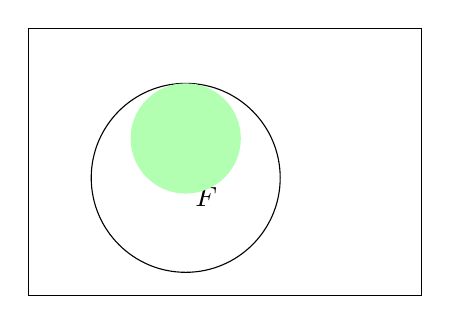
\begin{tikzpicture}[baseline]
        \draw (0,0) rectangle (5,3.4);
        \draw (2,1.5) circle (1.2cm) node[below right] {$F$};
        \fill[green!30] (2,2) circle (0.7cm) node[above] {$E$};
    \end{tikzpicture}
    &
    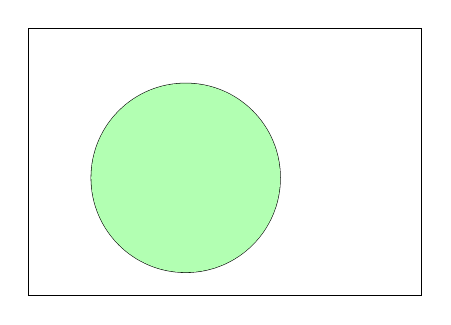
\begin{tikzpicture}[baseline]
        \draw (0,0) rectangle (5,3.4);
        \draw (2,1.5) circle (1.2cm) node[below right] {$F$};
        \fill[green!30] (2,1.5) circle (1.2cm) node[above] {$E$};
    \end{tikzpicture}
    &
    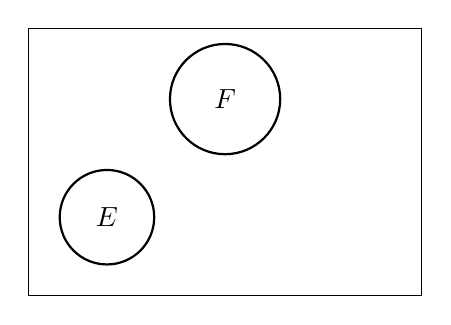
\begin{tikzpicture}[baseline]
        \draw (0,0) rectangle (5,3.4);
        \draw[thick] (1,1) circle (0.6cm) node {$E$};
        \draw[thick] (2.5,2.5) circle (0.7cm) node {$F$};
    \end{tikzpicture}
    \\
    
\end{tabular}
\end{center}

\section{What is Probability?}

There are three prominent ways to define probability.
In the three following subsections, these three definitions are explored.
Then an axiomatic definition of probability is given which is consistent with these three definitions.

\subsection{Classical Definition of Probability}\label{sec:classic}

In this definition, each elementary event of the sample space is considered to be equally likely to occur.
For example in rolling a fair die, all the events \( \{ 1 \}, \{ 2 \}, \{ 3 \}, \{ 4 \}, \{ 5 \} \) and \( \{ 6 \} \) have the same probability.
Or in tossing a coin (the random experiment in Example \autoref{exmp:coin_toss}), the elementary events \( \{ H \} \) and \( \{ T \} \) are all equally likely to happen,
which is consistent with our intuition of 50\% chance of occurring for each event.

This interpretation of probability goes back to Pierre-Simon Laplace, who wrote:
\begin{quote}
	The probability of an event is the ratio of the number of cases favorable to it, to the number of all cases possible when nothing leads us to expect that any one of these cases should occur more than any other, which renders them, for us, equally possible.
\FOOTNOTE{Laplace, Théorie analytique des probabilités, retrieved from \url{https://en.wikipedia.org/wiki/Classical_definition_of_probability}}
\end{quote}
So in this interpretation of probability, for an event \( E \subset S \), the probability of \( E \) is given by:
\begin{align*}
	P(E) = \frac{\text{number of outcomes in }E}{\text{total number of outcomes in }S}
\end{align*}

While we can assign a probability to each elementary event when the sample space consists of finitely many elements,
it is not possible when the elementary events are not equally likely to occur or the sample space is infinite like we saw in Example \autoref{exmp:heads_observe}.

\subsection{Frequentist Definition of Probability}

Consider a randon experiment in which we are interested in the occurrence of event \( E \).
Suppose this experiment is repeated \( n \) times under identical experimental conditions,
and event \( E \) occurs \( r \) times in total.
\( r \) and \( \frac{r}{n} \) are said to be the \keyterm{frequency} and \keyterm{relative frequency} of \( E \) in these
\( n \) trials, respectively.

As the number of trials \( n \) increases, the frequency \( r \) and consequently the relative frequency \( \frac{r}{n} \) changes as well.
However, empirical observations show that the relative frequency converges to a constant value, which in this interpretation is defined as the probability of \( E \).



The frequentist interpretation of probability may trace its earliest conceptual origins to Aristotle, who wrote
\begin{quote}
	the probable is that which for the most part happens
	\FOOTNOTE{Aristotle, Rhetoric, retrieved from \url{https://en.wikipedia.org/wiki/Frequentist_probability}}
\end{quote}
The frequentist interpretation of probability rose to dominance during the 19th century, becoming the foundation of classic statistical inference.

Let us reconsider the random experiment described in Example \autoref{exmp:three_balls_urn}.
According to the classical interpretation of probability, the probability of drawing a blue ball is \( \frac{1}{3} \).
However, if we don't know the urn's contents, we can determine the probability of drawing a red ball through a simple experiment.
By repeatedly drawing balls from the urn and calculating the relative frequency of drawing blue balls,
we observe that this ratio converges to \( \frac{1}{3} \) as the number of trials increases,
which is consistent with the classical definition of probabiltiy.
But the frequentist interpretation offers another advantage:
Suppose there are two blue balls, one green ball and one red ball in the urn.
Here, while the sample space remains \( \{ B, G, R \} \), the elementary events now have different probabilities
because there is an additional blue ball in the urn!
So while we cannot calculate the probability of drawing a blue ball using the classical definition,
we can determine it through the frequentist approach by performing many trials and observing the convergence of relative frequency.

While this interpretation sounds like a better approach to defining probability,
it faces several limitations. 
Consider, for instance, estimating the probability of precipitation occurring tomorrow.
There is, in fact, only one tomorrow;
we cannot conduct multiple trials of "tomorrow" to count rainy occurrences and determine their relative frequency.
Moreover, maintaining truly identical experimental conditions is practically impossible in most real-world scenarios.
Another fundamental challenge lies in determining how many trials are sufficient for the relative frequency to converge to a stable probability value.

\subsection{Epistemic Definition of Probability}

In this interpretation of probability, each observer assigns a subjective probability to an event based on their prior beliefs.
Reconsider the urn example from the previous subsection.
The experimenter draws a ball from the urn without revealing it to the observers.

An observer who saw the experimenter add an extra blue ball to the urn assigns a probability of \( \frac{2}{4} \) to the ball being blue.
Another observer, who previously knew the urn contained one blue, one green, and one red ball, assigns a probability of \( \frac{1}{3} \).
The experimenter, however, knows with certainty whether the ball is blue or not.

In the frequentist approach, the ball is either blue or not, and the probability is determined through repeated trials.
Thus, frequentists don't assign probabilities to single drawn balls.
In the epistemic perspective, however, each individual assigns a probability based on their existing knowledge.

\subsection{Axiomatic Definition of Probability}

Just like Euclidean geometry, where theorems are derived from a set of axioms taken as true\FOOTNOTE{\url{https://www.math.brown.edu/tbanchof/Beyond3d/chapter9/section01.html}},
modern probability theory is built upon axioms proposed by the Russian mathematician Andrey Kolmogorov in 1933.

A \keyterm{probability measure} on a sample space \( S \) is a function \( P(.) \) that assigns
to each event \( E \subset S \) a real number \( P(A) \), called the probability of \( A \),
satisfying the following three \keyterm{axioms of probability}:
\begin{itemize}
	\item for each event \( E \subset S \), the probability of \( A \) is non-negative, meaning \( P(E) \geq 0 \).
	\item the probability of \( S \) is 1, meaning \( P(S) = 1 \).
	\item if \( E_1, E_2, \ldots \) is a sequence of disjoint events, meaning \( E_i \cap E_j = \emptyset \) for each \( i \neq j \), then \( P(E_1 \cup E_2 \cup ...) = P(E_1) + P(E_2) + \ldots \).
\end{itemize}
The first axiom states that probabilities cannot be negative, which aligns with our intuition.
The second axiom indicates that since every experimental outcome belongs to the sample space, the event 
\( S \) must occur with probability 1.
The third axiom establishes that for any collection of disjoint events, the probability of their union equals the sum of their individual probabilities.

Different interpretations of probability remain consistent with the axiomatic definition.
Consider the frequentist approach:
\begin{itemize}
	\item Relative frequencies are non-negative, satisfying the first axiom.
	\item The relative frequency of \( S \) equals 1 in any number of trials, since every outcome belongs to the sample space.
	\item For mutually exclusive events, the relative frequency of their union equals the sum of their individual relative frequencies, as each outcome is counted only once.
\end{itemize}
Next, we prove some thorems using the axioms of probability.

\begin{theorem}\label{thm:imp_event}
	The probabiliy of impossible event, \( \emptyset \), is zero.
\end{theorem}
\begin{proof}
	Consider the sequence of events \( E_1, E_2, \ldots \) where \( E_1 = S \) and \( E_i = \emptyset \) for \( i > 1 \).
	Since the events in this sequence are mutually exclusive and \( S = \bigcup_{i = 1}^{\infty} E_i \), by the third axiom we have
	\[
	P(S) = P(\bigcup_{i = 1}^{\infty} A_i) = \sum_{i = 1}^{\infty} P(E_i) = P(S) + \sum_{i = 2}^{\infty} P(\emptyset) = P(S) + P(\bigcup_{i = 2}^{\infty}\emptyset) = P(S) + P(\emptyset)
	\]
	Cancelling \( P(S) \) from both sides we obtain \( P(\emptyset) = 0 \).
\end{proof}

\begin{theorem}\label{thm:finite_probs}
	For finitely many disjoint events \( E_1, E_2, \ldots, E_n \), we have
	\[
	P(\bigcup_{i = 1}^{n} E_i) = \sum_{i = 1}^{n} P(E_i)
	\]
\end{theorem}
\begin{proof}
	Consider the sequence of events \( E_1, E_2, \ldots \) where \( E_i = \emptyset \) for \( i > n \).
	Since all events in this sequence are mutually exclusive and \( \bigcup_{i = 1}^{n} E_i = \bigcup_{i = 1}^{\infty} E_i \),
	by applying the third axiom and \autoref{thm:imp_event} we have
	\begin{align*}
	P(\bigcup_{i = 1}^{n} E_i) = P(\bigcup_{i = 1}^{\infty} E_i) &= \sum_{i = 1}^{\infty} P(E_i)\\
	&= \sum_{i = 1}^{n} P(E_i) + \sum_{i = n + 1}^{\infty} P(E_i)\\
	&= \sum_{i = 1}^{n} P(E_i) + P(\bigcup_{i = n + 1}^{\infty} E_i)\\
	&= \sum_{i = 1}^{n} P(E_i) + P(\emptyset)\\
	&= \sum_{i = 1}^{n} P(E_i)
	\end{align*}
\end{proof}

\begin{theorem}
	For any event \( E \subset S \), \( P(E^\complement) = 1 - P(E) \).
\end{theorem}
\begin{proof}
	\( E \) and \( E^\complement \) are mutually exclusive and \( S = E \cup E^\complement \)
	since every element of the sample space is either in \( E \) or not.
	Thus, using the second axiom and \autoref{thm:finite_probs}, we have
	\begin{gather*}
		1 = P(S) = P(E \cup E^\complement) = P(E) + P(E^\complement)\\
		P(E^\complement) = 1 - P(E)
	\end{gather*}
\end{proof}
\begin{corollary}\label{cor:demorgan}
	Using De Morgan's laws in set theory, for any two events \( E, F \subset S \):
	\begin{align*}
		(E \cap F)^\complement = E^\complement \cup F^\complement\\
		(E \cup F)^\complement = E^\complement \cap F^\complement
	\end{align*}
	From these we can derive:
	\begin{align*}
		P(E^\complement \cup F^\complement) = P((E \cap F)^\complement) = 1 - P(E \cap F)\\
		P(E^\complement \cap F^\complement) = P((E \cup F)^\complement) = 1 - P(E \cup F)
	\end{align*}
\end{corollary}

\begin{theorem}\label{thm:difference_probs}
	For any two events \( F, E \subset S \), the equality \( P(F - E) = P(F) - P(E \cap F) \) holds.
\end{theorem}
\begin{proof}
	It can be shown that \( F = (F - E) \cup (E \cap F) \)
	where \( F - E \) and \( E \cap F \) are mutually exclusive.
	By \autoref{thm:finite_probs}:
	\begin{gather*}
		P(F) = P(F - E) + P(E \cap F)\\
		P(F - E) = P(F) - P(E \cap F)
	\end{gather*}
\end{proof}
\begin{corollary}\label{cor:subset_prob}
	If \( E \subset F \), then \( E \cap F = E \) and thus \( P(F - E) = P(F) - P(E) \).
\end{corollary}
\begin{corollary}
	If \( E \subset F \), the first axiom and Corollary \autoref{cor:subset_prob} yield \( P(E) \leq P(F) \).
	Replacing \( F \) with \( S \) and applying the second axiom gives \( P(E) \leq 1 \).
	Combined with the first axiom, this proves that for any event \( E \),
	\[
	0 \leq P(E) \leq 1
	\]
\end{corollary}

\begin{theorem}\label{thm:union_probs}
	For any two events \( E, F \subset S \), the equality \( P(E \cup F) = P(E) + P(F) - P(E \cap F) \) holds.
\end{theorem}
\begin{proof}
	It can be shown that \( E \cap F = E \cup (F - E) \)
	where \( E \) and \( F - E \) are mutually exclusive.
	By \autoref{thm:finite_probs} and \autoref{thm:difference_probs}:
	\[
		P(E \cup F) = P(E) + P(F - E) = P(E) + P(F) - P(E \cap F)
	\]
\end{proof}

\begin{exmp}
	Suppose \( E, F \) are two events from sample space \( S \) where \( P(E) = 0.6 \), \( P(F - E) = 0.3 \) and \( P(E \cap F) = 0.2 \).
	\begin{enumerate}
		\item What is \( P(F) \)?
		\item What is \( P(E \cup F) \)?
		\item What is \( P(E \cap F^\complement) \)?
		\item What is \( P(E \cap E^\complement) \)?
		\item What is \( P(E^\complement \cap F^\complement) \)?
	\end{enumerate}
\end{exmp}
\begin{solution}
	\begin{enumerate}
		\item From \autoref{thm:difference_probs}, we derive:
		\begin{align*}
			P(F) = P(F - E) + P(E \cap F) = 0.3 + 0.2 = 0.5
		\end{align*}
		\item By \autoref{thm:union_probs}:
		\begin{align*}
			P(E \cup F) = P(E) + P(F) - P(E \cap F) = 0.6 + 0.5 - 0.2 = 0.9
		\end{align*}
		\item From set theory, we have the equality \( E \cap F^\complement = E - F \).
		Intuitively, \( E \cap F^\complement \) and \( E - F \) both contain exactly those elements of \( S \) that belong to \( E \) but not to \( F \).
		Applying \autoref{thm:difference_probs} yields:
		\begin{align*}
			P(E \cap F^\complement) = P(E - F) = P(E) - P(F \cap E) = P(E) - P(E \cap F) = 0.6 - 0.2 = 0.4
		\end{align*}
		\item No element of \( S \) can simultaneously belong to \( E \) and not belong to it , thus \( E \cap E^\complement = \emptyset \).
		\autoref{thm:imp_event} implies:
		\begin{align*}
			P(E \cap E^\complement ) = P(\emptyset) = 0
		\end{align*}
		\item By Corollary \autoref{cor:demorgan}:
		\begin{align*}
			P(E^\complement \cap F^\complement) = 1 - P(E \cup F) = 1 - 0.9 = 0.1
		\end{align*}
	\end{enumerate}
\end{solution}

\begin{ex}
	Show that for any two events \( E, F \subset S \), \( P(E^\complement \cup F) = 1 - P(E) + P(F \cap E) \).
\end{ex}
\begin{ex}\label{ex:marginal_probs}
	Suppose \( E, F \) are two events of sample space \( S \).
	\begin{enumerate}
		\item Show that \( P(E \cap F) + P(E \cap F^\complement) = P(E) \).
		\item Show that \( P(E) + P(E^\complement) = 1 \).
	\end{enumerate}
\end{ex}

\section{Uniform Probability Model}

In a \keyterm{uniform probability model}, each elementary event has an equal probability.
So if the sample space has \( n(S) \) elements, then for each outcome \( e_i \in S \), we have:
\begin{align*}
	P(\{e_i\}) = \frac{1}{n(S)}
\end{align*}
If an event \( E \) contains \( n(E) \) elements,
we can express it as \( E = \bigcup_{j} \{e_j\} \), where each \( e_j \) is an element of \( S \) belonging to \( E \).
Applying \autoref{thm:finite_probs}:
\begin{align*}
	P(E) = P(\bigcup_{j} \{e_j\}) = \sum_{j} P(\{e_j\}) = \sum_{j} \frac{1}{n(S)} = \frac{n(E)}{n(S)}
\end{align*}
Comparing this with \autoref{sec:classic}, we observe that it is equivalent to Laplace's classical definition of probability.

\begin{exmp}
	In the coin toss random experiment from Example \autoref{exmp:coin_toss}, if the event of interest \( E \) is "observing heads",
	then \( P(E) = \frac{1}{2} \), since \( E = \{ H \} \) contains exactly one outcome out of two possible equally likely outcomes.
	Such a coin with equal probabilities of landing on heads or tails is called a \keyterm{fair coin}.
\end{exmp}

\begin{exmp}\label{exmp:three_fair_coins}
	In the random experiment of tossing three fair coins, the sample space is
	\( S = \{ HHH, HHT, HTH, HTT, THH, THT, TTH, TTT \} \).
	If the event of interest \( E \) is "observing at most two heads",
	then \( E = \{ HHT, HTH, HTT, THH, THT, TTH, TTT \} \) and consequently \( P(E) = \frac{7}{8} \).
\end{exmp}

\begin{exmp}
	In the die-throw random experiment from Example \autoref{exmp:fair_die}, if the event of interest \( E \) is "observing an odd number",
	then \( E = \{ 1, 3, 5 \} \) and thus \( P(E) = \frac{3}{6} = \frac{1}{2} \).
	A die with equally likely outcomes for all faces is called a \keyterm{fair die}.
\end{exmp}

\begin{exmp}\label{exmp:two_fair_dice}
	In the random experiment of tossing two fair six-sided dice, the sample space is
	\( S = \{ (1, 1), (1, 2), \ldots, (6, 5), (6, 6) \} \).
	If the event of interest \( E \) is "the sum of two dice equals 8",
	then \( E = \{ (2, 6), (3, 5), (4, 4), (5, 3), (6, 2) \} \) and consequently \( P(E) = \frac{5}{36} \).
\end{exmp}

\begin{ex}
	In Example \autoref{exmp:two_fair_dice}, what is the probability that the difference of two dice is 3?
\end{ex}

In the examples discussed above, we can easily count the elements in both the sample space and the event of interest.
However, consider modifying Example \autoref{exmp:three_fair_coins} where six fair coins are tossed instead of three,
or altering Example \autoref{exmp:two_fair_dice} to involve seven fair six-sided dice rather than two.
How many elements are in the sample space in these cases?
Attempting to list all possible combinations would quickly reveal what a tedious task this becomes.

The are some fundamental counting principles which aid us in these scenarios.
The \keyterm{multiplication principle} states that if a first task can be performed in \( m_1 \) ways,
and for each of these, a second task can be performed in \( m_2 \) ways independent from the previous task,
then the sequence of two tasks has \( m_1 \times m_2 \) possible outcomes.
This naturally extends to \( n \) sequential tasks,
where the total number of possible outcomes becomes \( m_1 \times m_2 \times \ldots \times m_n \).

\begin{exmp}
	A standard deck contains cards with four suits (\( \clubsuit, \vardiamondsuit, \spadesuit, \varheartsuit \)) and thirteen ranks (A, 1, 2, ..., 9, J, Q, K).
	How many total cards are in such a deck?
\end{exmp}
\begin{solution}
	We decompose the counting problem into two sequential tasks:
	selecting a suit and then selecting a rank.
	There are four ways to do the former and thirteen ways to do the latter, so in total there are \( 4 \times 13 = 52 \) such cards.
\end{solution}

The \keyterm{addition principle} states that if one task can be performed in \( n_1 \) ways and another distinct task in \( n_2 \) ways,
then either task can be done in \( n_1 + n_2 \) total ways.
For example, with three blue garments and seven green ones,
selecting either a blue or green garment can be done in \( 3 + 7 = 10 \) ways.
This result can be generalized to more than two tasks, analogous to the extension of the multiplication principle.

\begin{exmp}
	From a group of seven statisticians and five computer scientists, two people are randomly selected for a project.
	What is the probability that the team consists of one statistician and one computer scientist?
\end{exmp}
\begin{solution}
	The first person is chosen from 12 individuals, and the second from the remaining 11.
	So the sample space has \( n(S) = 12 \times 11 = 132 \) elements.
	The event \( E \) contains elements of \( S \) with one statistician and one computer scientist.
	So to count the number of elements in \( E \), we again decompose the problem into two tasks.
	First choosing one statistician and second choosing a conputer scientist,
	which can be done in \( 7 \times 5 = 35 \) ways.
	Or first choosing one computer scientist and then choosing a statistician,
	which can be done in \( 5 \times 7 = 35 \) ways.
	Since we have to choose a statistician first and then a computer scientist, or first a computer scientist and then a statistician,
	the addition principle implies \( n(E) = 35 + 35 = 70 \), yielding \( P(E) = \frac{70}{132} = \frac{35}{66} \).
\end{solution}

\section{Conditional Probability}

In previous sections, we examined basic probability examples.
But sometimes in our problems, we have some prior information.
In Example \autoref{exmp:two_fair_dice}, suppose we know beforehand that one die has come up 2.
Here, the event of interest becomes \( E \cap F \), where \( F \) is the event "one die comes up 2".
So we are interested in the probability of both \( E \) and \( F \) occurring, which is \( E \cap F = \{ (2, 6), (6, 2) \} \).
On the other hand, since we have information that one die has come up 2, the sample space is restricted from \( S \) to \( F \).
So the probability of \( E \) given we know \( F \) has occurred is \( \frac{n(E \cap F)}{n(F)} \).
By dividing the numerator and denominator by \( n(S) \), the desired probability becomes \( \frac{P(E \cap F)}{P(F)} \).
Since \( F = \{ (1, 2), (2, 1), (2, 2), (2, 3), (2, 4), (2, 5), (2, 6), (3, 2), (4, 2), (5, 2), (6, 2) \} \),
this probability is \( \frac{\frac{2}{36}}{\frac{11}{36}} = \frac{2}{11} \).

The \keyterm{conditional probability} of \( E \) given \( F \) is defined the same way in any probability model, not just the uniform one, and is denoted by \( P(E | F) = \frac{P(E \cap F)}{P(F)} \)
where \( P(F) > 0 \).
If \( P(F) = 0 \), \( P(E | F) \) would be undefined.

\begin{exmp}
	In Example \autoref{exmp:three_fair_coins}, let \( F \) be the event "observing exactly two tails".
	\begin{enumerate}
		\item What is \( P(E \cap F) \)?
		\item What is \( P(E | F) \)?
		\item What is \( P(F | E) \)?
	\end{enumerate}
\end{exmp}
\begin{solution}
	\begin{enumerate}
		\item First we note that \( F = \{ HTT, THT, TTH \} \).
		Thus, \( E \cap F = \{ HTT, THT, TTH \} \), yielding:
		\begin{align*}
			P(E \cap F) = \frac{n(E \cap F)}{n(S)} = \frac{3}{8}
		\end{align*}
		Here, we are interested in the event "observing at most two heads and exactly two tails" while the sample space is not restricted to a new one since we have no prior information.
		\item \begin{gather*}
			P(F) = \frac{n(F)}{n(S)} = \frac{3}{8}\\
			P(E | F) = \frac{P(E \cap F)}{P(F)} = \frac{\frac{3}{8}}{\frac{3}{8}} = 1
		\end{gather*}
		Unlike the previous part, we now have prior information that exactly two tails are observed. 
		By restricting our sample space to outcomes with exactly two tails, we are sure that zero or one head must be observed (and thus at most two heads total), which agrees with this result.
		\item \begin{gather*}
			P(F | E) = \frac{P(F \cap E)}{P(E)} = \frac{P(E \cap F)}{P(E)} = \frac{\frac{3}{8}}{\frac{7}{8}} = \frac{3}{7}
		\end{gather*}
		Let \( G \) be the event "observing at least one tail".
		Since \( G = E \), the two events are equal and so \( P(F | E) = P(F | G) \).
		In other words, \( P(F | E) \) is the same as the probability of observing exactly two tails given at least one tail is observed.
		The plausibility of observing exactly two tails after at least one tail is observed must increase,
		which is true since \( P(F | E) = \frac{3}{7} > \frac{3}{8} = P(F) \).
	\end{enumerate}
\end{solution}

Thus far, we have examined numerous examples of uniform probability models.
However, not all probability models are uniform.
Consider these cases:

\begin{exmp}
	Consider Example \autoref{exmp:three_balls_urn} with an urn containing three blue balls, five green balls, and two red balls.
	If we treat each ball as distinct, the sample space is \( S = \{ B_1, B_2, B_3, G_1, G_2, G_3, G_4, G_5, R_1, R_2 \} \).
	This forms a uniform probability model where \( P(\{B_1\}) = P(\{B_2\}) = \ldots = P(\{R_1\}) = P(\{R_2\}) = \frac{1}{10} \).
	However, if we are only interested in ball colors and not individual balls,
	the sample space reduces to \( S = \{ B, G, R \} \).
	Defining \( B = \{ B_1, B_2, B_3 \} \), \( G = \{ G_1, G_2, G_3, G_4, G_5 \} \) and \( R = \{ R_1, R_2 \} \),
	then \( P(B) = \frac{3}{10} \), \( P(G) = \frac{5}{10} = \frac{1}{2} \) and \( P(R) = \frac{2}{10} = \frac{1}{5} \),
	which is a non-uniform probability model.
\end{exmp}

\begin{exmp}\label{exmp:eye_color}
	The residents of a town have blue, green, brown, and amber eyes.
	When randomly selecting a resident, the event of interest is their eye color.
	The sample space for this experiment is \( S = \{ blue, green, brown, amber \} \).
	To determine the probabilities of elementary events, we conduct a survey by randomly sampling 500 people and recording their eye colors.
	The results are shown in the following table:
	\begin{center}
	\begin{tabular}{|l|r|r|r|r|r|}
	\hline
	\textbf{Eye Color} & \textbf{Blue} & \textbf{Green} & \textbf{Brown} & \textbf{Amber} & \textbf{Total} \\ 
	\hline
	Frequency & 125 & 65 & 290 & 20 & 500 \\
	Relative Frequency & 0.25 & 0.13 & 0.58 & 0.04 & 1.00 \\
	\hline
	\end{tabular}
	\end{center}
	{\footnotesize\textit{Note: Data reflects approximate global eye color distribution based on studies from the American Academy of Ophthalmology (2022)\FOOTNOTE{\url{https://www.aao.org/eye-health/tips-prevention/your-blue-eyes-arent-really-blue}}.}}
	
	Using the frequentist definition of probability and the survey data above, we obtain:
	\begin{align*}
		P(\{blue\}) = 0.25, P(\{green\}) = 0.13, P(\{brown\}) = 0.58, P(\{amber\}) = 0.04
	\end{align*}
	These unequal probabilities confirm this is not a uniform probability model.

	Using this model, we can answer questions like this:
	If there are 362500 residents in this town, how many are expected to have green eyes?
	
	Using the frequentist interpretation, we can answer this question through a simple calculation:
	\begin{align*}
		0.13 \times 362500 = 47125
	\end{align*}
\end{exmp}

The conditional probability and theorems derived from the three axioms of probability apply to any probability model.
The following example demonstrates this:

\begin{exmp}
	Suppose in Example \autoref{exmp:eye_color}, of people with blue eyes, 65 were female.
	One person is selected at random from the town.
	Given that the selected person has blue eyes, what is the probability that they are female?
\end{exmp}
\begin{solution}
	We define event \( E \) as "the selected pesron has blue eyes" and event \( F \) as "the selected person is female".
	Thus:
	\begin{gather*}
		P(F \cap E) = \frac{65}{500} = 0.13\\
		P(F | E) = \frac{P(F \cap E)}{P(E)} = \frac{0.13}{0.25} = 0.52
	\end{gather*}
\end{solution}

\section{Contingency Tables}

When solving conditional probability problems, visual tools like tree diagrams and contingency tables often give invaluable insights.
These complementary techniques provide different perspectives that can clarify complex probability relationships.

Contingency tables are particularly useful when analyzing two events, say \( E, F \subset S \).
We can construct contingency tables using the size of events as follows:
\begin{center}
\begin{tabular}{l|cc|c}
                       & \( E \) & \( E^\complement \) &  \\ \hline
\( F \)                & \( n(E \cap F) \) & \( n(E^\complement \cap F) \) & \( n(F) \) \\ 
\( F^\complement \)    & \( n(E \cap F^\complement) \) & \( n(E^\complement \cap F^\complement) \) & \( n(F^\complement) \) \\ \hline
                       & \( n(E) \) & \( n(E^\complement) \) & \( n(S) \)
\end{tabular}
\end{center}
Note that the sizes in margins of the table are computed by summing the respective row or column entries. 
For instance, in the first column, \( n(E) = n(E \cap F) + n(E \cap F^\complement) \),
since elements in \( E \) must belong to either \( F \) or \( F^\complement \).

This table can also be constructed using probabilities:
\begin{center}
\begin{tabular}{l|cc|c}
                       & \( E \) & \( E^\complement \) &  \\ \hline
\( F \)                & \( P(E \cap F) \) & \( P(E^\complement \cap F) \) & \( P(F) \) \\ 
\( F^\complement \)    & \( P(E \cap F^\complement) \) & \( P(E^\complement \cap F^\complement) \) & \( P(F^\complement) \) \\ \hline
                       & \( P(E) \) & \( P(E^\complement) \) & \( P(S) = 1 \)
\end{tabular}
\end{center}
Note that in this table, the marginal probabilities are again the sum of their respective row or column entries,
which can be verified using Exercise \autoref{ex:marginal_probs}.

\begin{exmp}
	A study was conducted to find the relationship between dog ownership (D) and cat ownership (C) among pet owners in the U.S.
	In a sample of 300 American pet owners, the researchers found that 219 owned dogs,
	12 had neither cats nor dogs,
	and 72 owned both cats and dogs.\FOOTNOTE{based on data from \url{https://pewrsr.ch/3JPtwoR}}
	\begin{enumerate}
		\item Construct a contingency table for cat and dog owners.
		\item Find \( P(C \cap D) \).
		\item Find \( P(C^\complement) \).
		\item Find \( P(D | C^\complement) \).
	\end{enumerate}
\end{exmp}
\begin{solution}
	\begin{enumerate}
		\item From the information given in the problem statement:
		\begin{center}
		\begin{tabular}{l|cc|c}
							& \( D \) & \( D^\complement \) &  \\ \hline
		\( C \)                & 72 & & \\ 
		\( C^\complement \)    & & 12 &  \\ \hline
							& 219 &  & 300
		\end{tabular}
		\end{center}
		Completing the remaining entries in the table yields:
		\begin{center}
		\begin{tabular}{l|cc|c}
							& \( D \) & \( D^\complement \) &  \\ \hline
		\( C \)                & 72 & 69 & 141 \\ 
		\( C^\complement \)    & 147 & 12 & 159  \\ \hline
							& 219 & 81 & 300
		\end{tabular}
		\end{center}
		\item Using the frequentist interpretation of probability and the contingency table results, we derive:
		\begin{align*}
			P(C \cap D) = \frac{n(C \cap D)}{n(S)} = \frac{72}{300} = 0.24
		\end{align*}
		\item \begin{align*}
			P(C^\complement) = \frac{n(C^\complement)}{n(S)} = \frac{159}{300} = 0.53
		\end{align*}
		\item \begin{gather*}
			P(D \cap C^\complement) = \frac{n(D \cap C^\complement)}{n(S)} = \frac{147}{300} = 0.49\\
			P(D | C^\complement) = \frac{P(D \cap C^\complement)}{P(C^\complement)} = \frac{0.49}{0.53} \approx 0.92
		\end{gather*}
		Hence, it is highly probable that pet owners without cats prefer dogs over other pets.

		Another way to calculate \( P(D | C^\complement) \) is:
		\begin{align*}
			P(D | C^\complement) = \frac{P(D \cap C^\complement)}{P(C^\complement)} = \frac{\frac{n(D \cap C^\complement)}{n(S)}}{\frac{n(C^\complement)}{n(S)}} = \frac{n(D \cap C^\complement)}{n(C^\complement)} = \frac{147}{159} \approx 0.92
		\end{align*}
	\end{enumerate}
\end{solution}
\begin{ex}
	In the previous exercise, find \( P(C | D^\complement) \), compare it with \( P(D | C^\complement) \) and interpret the results.
\end{ex}

\section{Independent Events}

Suppose \( E \) and \( F \) are two events with positive probabilities.
It is possible that prior information that \( F \) has occurred does not affect the occurrence of \( E \), or in other words:
\begin{align*}
	P(E | F) = P(E)
\end{align*}
If this is the case, we say \( E \) is independent of \( F \).
Next, we show that if \( E \) is independent of \( F \), \( F \) is also independent of \( E \).

By definition, \( P(E | F) = \frac{P(E \cap F)}{P(F)} \) which implies \( P(E \cap F) = P(E | F)P(F) \).
Since \( E \) is independent of \( F \), we have \( P(E | F) = P(E) \), and consequently:
\begin{align*}
	P(F | E) = \frac{P(F \cap E)}{P(E)} = \frac{P(E \cap F)}{P(E)} = \frac{P(E | F)P(F)}{P(E)} = \frac{P(E)P(F)}{P(E)} = P(F)
\end{align*}
An additional observation from \( P(E | F) = P(E) \) is:
\begin{gather*}
	P(E | F) = P(E) = \frac{P(E \cap F)}{P(F)}\\
	P(E \cap F) = P(E)P(F)
\end{gather*}
We therefore define \( E \) and \( F \) as \keyterm{independent events} if any of the following equivalent conditions hold:
\begin{itemize}
	\item \( P(E | F) = P(E) \)
	\item \( P(F | E) = P(F) \)
	\item \( P(E \cap F) = P(E)P(F) \)
\end{itemize}

\section{Bayes' Theorem}

In this section we see an important formula which utilizes conditional probability.
Before that, we discuss some important prerequisites.

\subsection{Partitioning the sample space into mutually exclusive events}

Suppose events \( E_1, E_2, \ldots, E_k \) with positive probabilities are mutually exclusive and their union is the sample space, \( S \).
In other words,
\begin{gather*}
	E_i \cap E_j = \emptyset
\end{gather*}
for \( i \neq j \) where \( i, j = 1, 2, \ldots k \), and
\begin{gather*}
	\bigcup_{i = 1}^{k} E_i = S
\end{gather*}
In this case, we say \( S \) is partitioned into these events.

\begin{exmp}
	We can partition the sample space in Example \autoref{exmp:three_fair_coins} to events "zero heads", "one head", "two heads" and "three heads" as follows:
	\begin{gather*}
		\{ TTT \}, \{ HTT, THT, TTH \}, \{ HHT, HTH, THH \}, \{ HHH \}
	\end{gather*}
\end{exmp}

\subsection{Partitioning an event into mutually exclusive events}

Suppose \( S \) is partitioned into events \( E_1, E_2, \ldots, E_k \).
For any other event \( F \) with positive probability we have:
\begin{gather*}
	F = S \cap F = (\bigcup_{i = 1}^{k} E_i) \cap F = \bigcup_{i = 1}^{k} (E_i \cap F)
\end{gather*}
In this case, we say \( F \) is partitioned into events \( F \cap E_1, F \cap E_2, \ldots, F \cap E_k \).
Note that since \( E_1, E_2, \ldots, E_k \) are mutually exclusive, \( F \cap E_1, F \cap E_2, \ldots, F \cap E_k \) are also disjoint events.
This is also illustrated in \autoref{fig:event_partitioning}.
In this figure, \( B \) is partitioned into three events \( A_1 \cap B, A_2 \cap B, \text{ and } A_3 \cap B \).
\begin{figure}[t]
\begin{center}
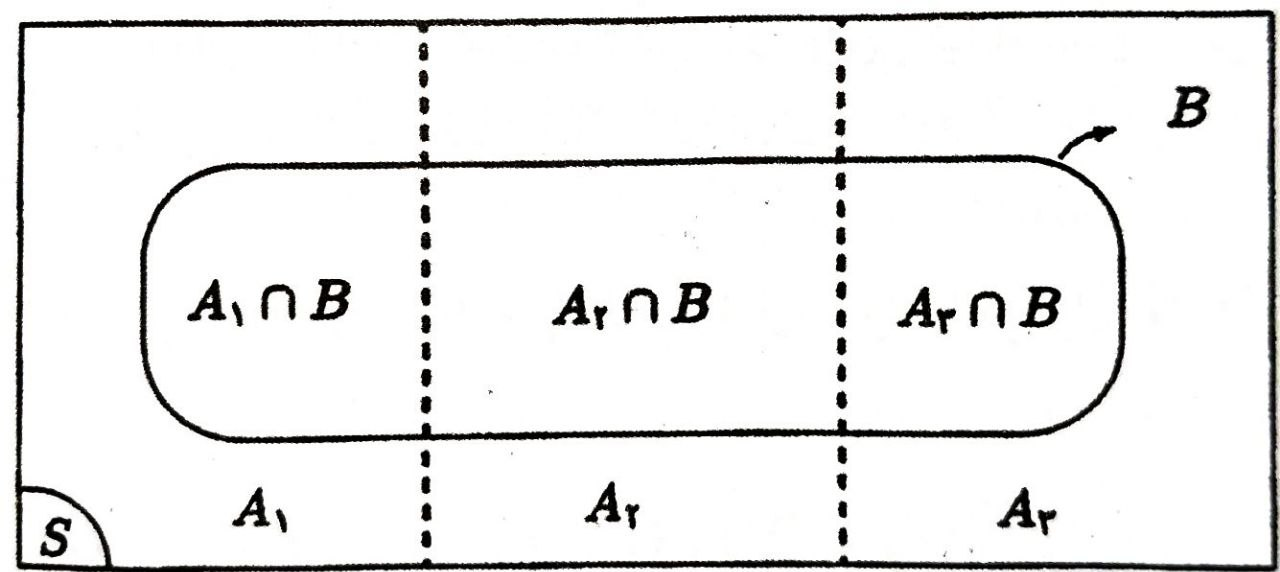
\epsfig{file=../img/event_partitioning.jpg,clip=true,width=8.8cm}
\end{center}
\caption{Partitioning event \( B \) into three events}
\label{fig:event_partitioning}
%\HR
\end{figure}

\begin{exmp}
	Consider an experiment where a card is drawn at random from a deck numbered from 1 to 20.
	Suppose the sample space \( S \) is partitioned into two events:
	\begin{enumerate}
		\item \( E \): drawing an even-numbered card
		\item \( O \): drawing an odd-numbered card
	\end{enumerate}
	Then, the event \( A \), "drawing a multiple of 5", can be partitioned into two events:
	\begin{enumerate}
		\item \( A \cap O = \{ 5, 15 \} \) (odd multiples of 5)
		\item \( A \cap E = \{ 10, 20 \} \) (even multiples of 5)
	\end{enumerate}
\end{exmp}

\subsection{Law of Total Probability}

If \( F \) is partitioned into events \( E_1, E_2, \ldots, E_n \), then \autoref{thm:finite_probs} yields:
\begin{gather*}
	P(F) = P(\bigcup_{i = 1}^{k} (E_i \cap F)) = \sum_{i = 1}^{k} P(E_i \cap F)
\end{gather*}
Since \( P(F | E_i) = \frac{P(F \cap E_i)}{P(E_i)} \), we can alternatively write the above formula as:
\begin{gather*}
	P(F) = P(\bigcup_{i = 1}^{k} (F \cap E_i)) = \sum_{i = 1}^{k} P(F | E_i)P(E_i)
\end{gather*}
which is called \keyterm{the law of total probability}.

\subsection{Bayes' Rule}

From the definition of conditional probability we know:
\begin{gather*}
	P(E_j | F) = \frac{P(E_j \cap F)}{P(F)}
\end{gather*}
where \( j = 1, 2, \ldots, k \).

Utilizing the law of total probability in the ablove formula yields:
\begin{gather*}
	P(E_j | F) = \frac{P(F | E_j)P(E_j)}{\sum_{i = 1}^{k}P(F | E_i)P(E_i)}
\end{gather*}
This result is known as \keyterm{Bayes' rule},
which provides a method for computing conditional probabilities when the sample space is partitioned into mutually exclusive events.

\begin{exmp}
	We have three boxes.
	The first box contains two black marbles and one red marble,
	the second contains two red marbles and two black marbles,
	and the third contains three black marbles and two red marbles.
	Assume the boxes and marbles differ only in their colors and identities.
	We randomly select one box and then draw one marble from it.
	\begin{enumerate}
		\item What is the probability that the drawn marble is black?
		\item Given that the drawn marble is black, what is the probability that it came from third box?
	\end{enumerate}
\end{exmp}
\begin{solution}
	A box is chosen and then a marble is drawn from that box.
	The sample space is \( S = \{ B_1, B_2, R_1, R_2, R_3, B_3, B_4, B_5, B_6, B_7, R_4, R_5 \} \) since no two marbles are identical.
	\( S \) is partitioned into three events depending on the three boxes containing the marbles:
	\( A_1, A_2, \text{ and } A_3 \), where \( A_1 = \{ B_1, B_2, R_1 \}, A_2 = \{ R_2, R_3, B_3, B_4 \}, \text{ and } A_3 = \{ B_5, B_6, B_7, R_4, R_5 \} \).
	In other words, \( A_i \) represents the event that the chosen box is the \( i \)th box and so the marble drawn would be an element of \( A_i \).
	There are no restrictions on choosing any box, and so the best model is a uniform probability model.
	Thus:
	\begin{gather*}
		P(A_1) = P(A_2) = P(A_3) = \frac{1}{3}
	\end{gather*}
	Suppose \( B \) is the event "the marble drawn from the chosen box is black".
	Depending on the chosen box, there are three cases to consider:
	\begin{gather*}
		P(B | A_1) = \frac{2}{3}, P(B | A_2) = \frac{2}{4} = \frac{1}{2}, P(B | A_3) = \frac{3}{5}
	\end{gather*}
	Let us analyze this more thoroughly:
	for example, suppose the chosen box is the second one.
	This means that the sample space is reduced to \( A_2 = \{ R_2, R_3, B_3, B_4 \} \), and hence the event "choosing a black marble" is \( \{ B_3, B_4 \} \).
	\begin{enumerate}
		\item By the law of total probability:
		\begin{align*}
			P(B) &= P(B | A_1)P(A_1) + P(B | A_2)P(A_2) + P(B | A_3)P(A_3)\\
			&= (\frac{2}{3})(\frac{1}{3}) + (\frac{1}{2})(\frac{1}{3}) + (\frac{3}{5})(\frac{1}{3}) = \frac{53}{90}
		\end{align*}
		\item By the Bayes' rule:
		\begin{align*}
			P(A_3 | B) = \frac{P(B | A_3)P(A_3)}{P(B)} = \frac{(\frac{3}{5})(\frac{1}{3})}{\frac{53}{90}} = \frac{18}{53}
		\end{align*}
	\end{enumerate}
\end{solution}

\section{Sensitivity, Specificity, Prevalence, and Relative Risk}

The importance of Bayes' Theorem is probably best understood through biomedical scenarios.
Consider a disease and a test developed for it which determines whether a patient has that disease or not.
Suppose a patient does the test, and the test is either positive or negative.
But there is uncertainty involved here:
the test does not always accurately identify the presence or absence of the disease.

Define \( T \) as the event that "the test is positive".
So \( T^\complement \) is the event that "the test is negative".
We also define \( D \) as the event that "the patient has the disease".
Now in case \( P(T | D) \) and \( P(T^\complement | D^\complement) \) are given,
the probabilty that the patient has the disease if their test is positive can be calculated using the Bayes' rule:
\begin{gather*}
	P(D | T) = \frac{P(T | D)P(D)}{P(T | D)P(D) + P(T | D^\complement)P(D^\complement)}
\end{gather*}
where \( P(T | D^\complement) = 1 - P(T^\complement | D^\complement) \) (why?).

\( P(T | D) \) is called \keyterm{sensitivity} of the test, and \( P(T^\complement | D^\complement) \) the \keyterm{specificity} of it.
In other words, sensitivity is the probability that the test correctly identifies patients who have the disease,
and specificity the probability that the test correctly identifies those who do not have the disease.

These terms can be used in a more general binary classification framework and are not restricted to biomedical applications.
Consider an algorithm developed to categorize emails as "spam" or "not spam".
Within this framework, we must clearly define what constitutes a positive and negative result.
For instance, one researcher might classify "spam" as positive and "not spam" as negative, while another could adopt the opposite convention.
The emails that are correctly identified as positive are called \keyterm{true positives},
and the ones that are correctly identified as negative are called \keyterm{true negatives}.
On the other hand, those falsely identified as positives are called \keyterm{false positives},
and those falsely identified as negatives, \keyterm{false negatives}.
The probability that this algorithm identifies true positives correctly is sensitivity or equivalently true positive rate,
and the probability that it identifies true negatives is specificity or equivalently true negative rate.

\begin{exmp}
	Suppose we define "spam" as positive and "non-spam" as negative.
	An algorithm with 90\% sensitivity correctly identifies 90 out of 100 actual spams as spam (true positives), and misclassifies 10 as non-spam (false negatives).
\end{exmp}

\begin{exmp}
	Consider an HIV test that classifies HIV-positive cases as positive and HIV-negative cases as negative.
	With 97\% specificity, the test correctly identifies 97 out of 100 truly HIV-negative individuals as negative (true negatives),
	while incorrectly classifying 3 as positive (false positives).
\end{exmp}

\begin{exmp}
	Developers at a food company have created a sentiment analysis algorithm that classifies customer feedback as either "satisfied" (positive) or "dissatisfied" (negative).
	From a test dataset of 500 comments, 200 were known to be from satisfied customers and 300 from dissatisfied customers.
	The algorithm classified 150 of the true satisfied comments correctly as positive,
	but incorrectly labeled 20 of the dissatisfied comments as positive.
	Using these results, calculate the algorithm's sensitivity and specificity.
\end{exmp}
\begin{solution}
	We first create a contingency table based on the data:
	\begin{center}
	\begin{tabular}{l|cc|c}
						& \( H \) & \( H^\complement \) &  \\ \hline
	\( P \)                & 150 & 20 & 170\\ 
	\( P^\complement \)    & 50 & 280 & 330 \\ \hline
						& 200 & 300 & 500
	\end{tabular}
	\end{center}
	where \( H \) is the event "customer is satisfied" and \( P \) the event "comment is labeled as positive".
	Sensitivity is calculated as:
	\begin{gather*}
		P(P | H) = \frac{P(P \cap H)}{P(H)} = \frac{\frac{150}{500}}{\frac{200}{500}} = 0.75
	\end{gather*}
	and specificity as:
	\begin{gather*}
		P(P^\complement | H^\complement) = \frac{P(P^\complement \cap H^\complement)}{P(H^\complement)} = \frac{\frac{280}{500}}{\frac{300}{500}} \approx 0.93
	\end{gather*}
\end{solution}